\subsection{User interfaces} % aka "Ease of use"
As stated in section \ref{sec:usability} and subsection \ref{subsec:user_interfaces} the application's UI must be extremely user-friendly and functionally equivalent across devices. 
\\Regarding the mobile UI a 3-page mockup is presented (fig. \ref{fig:mobile_mockup}) to highlight the most important functions: 
\begin{figure}[!ht]
	\centering
	\vspace{0.2cm}
	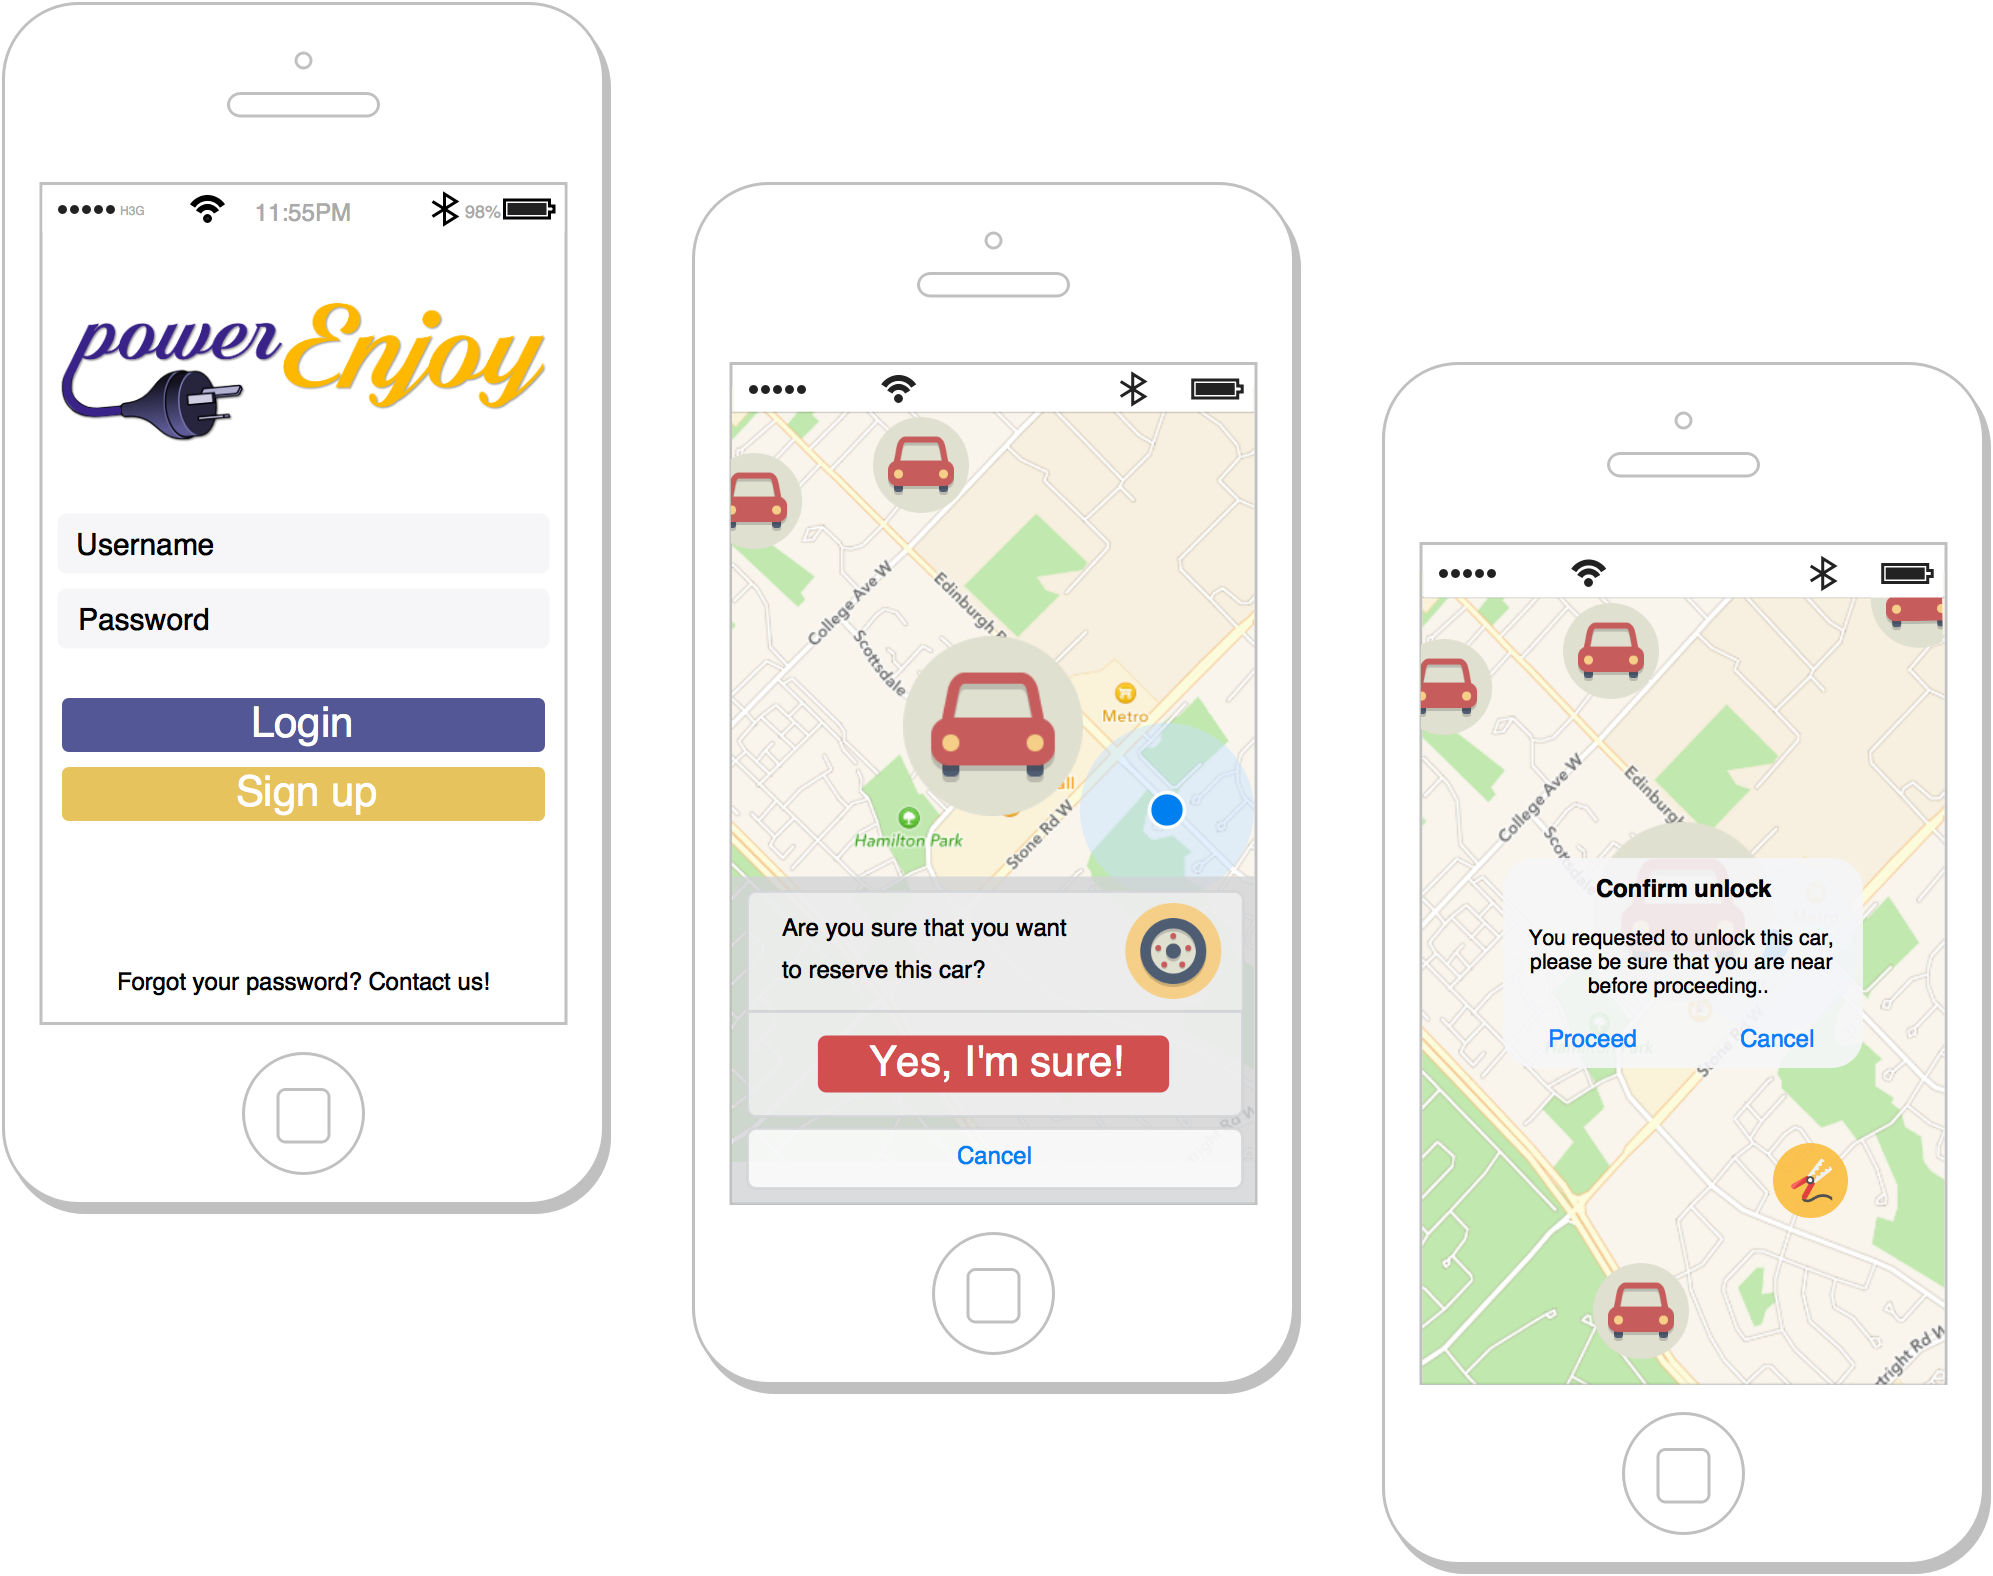
\includegraphics[width=1.0\textwidth]{/RASD/mobile_mockup}\\ 
	\vspace{0.5cm}
	\caption{3-page mockup representing the main pages of the mobile application} \label{fig:mobile_mockup} 
\end{figure}
\begin{itemize}
	\item{Login: the first page presented to the end-user is a simple login/signup page where she can login using her credentials or register to the system}
	\item{Car reservation and localization: this is probably the most important use-case, the user will be able to browse and find nearby cars, eventually requesting a reservation}
	\item{Unlock: the user will request to unlock the car through a procedure similar to the one described in point 2 above; she must submit the car PIN code displayed on the vehicle's windscreen, then a confirmation will be asked to enforce security and advise the user to really locate the car before unlocking it}
\end{itemize}

\bigskip
Additional in-detail mockups are presented in section \ref{sec:system_functions} along with the use-cases specification.
\bigskip

The web application will be really similar in features to the mobile application, the main use-cases are in fact the ones presented above in figure \ref{fig:mobile_mockup}; a basic mockup is presented (fig. \ref{fig:web_mockup}) to provide completeness:
\begin{figure}[!ht]
	\centering
	\vspace{0.2cm}{}
	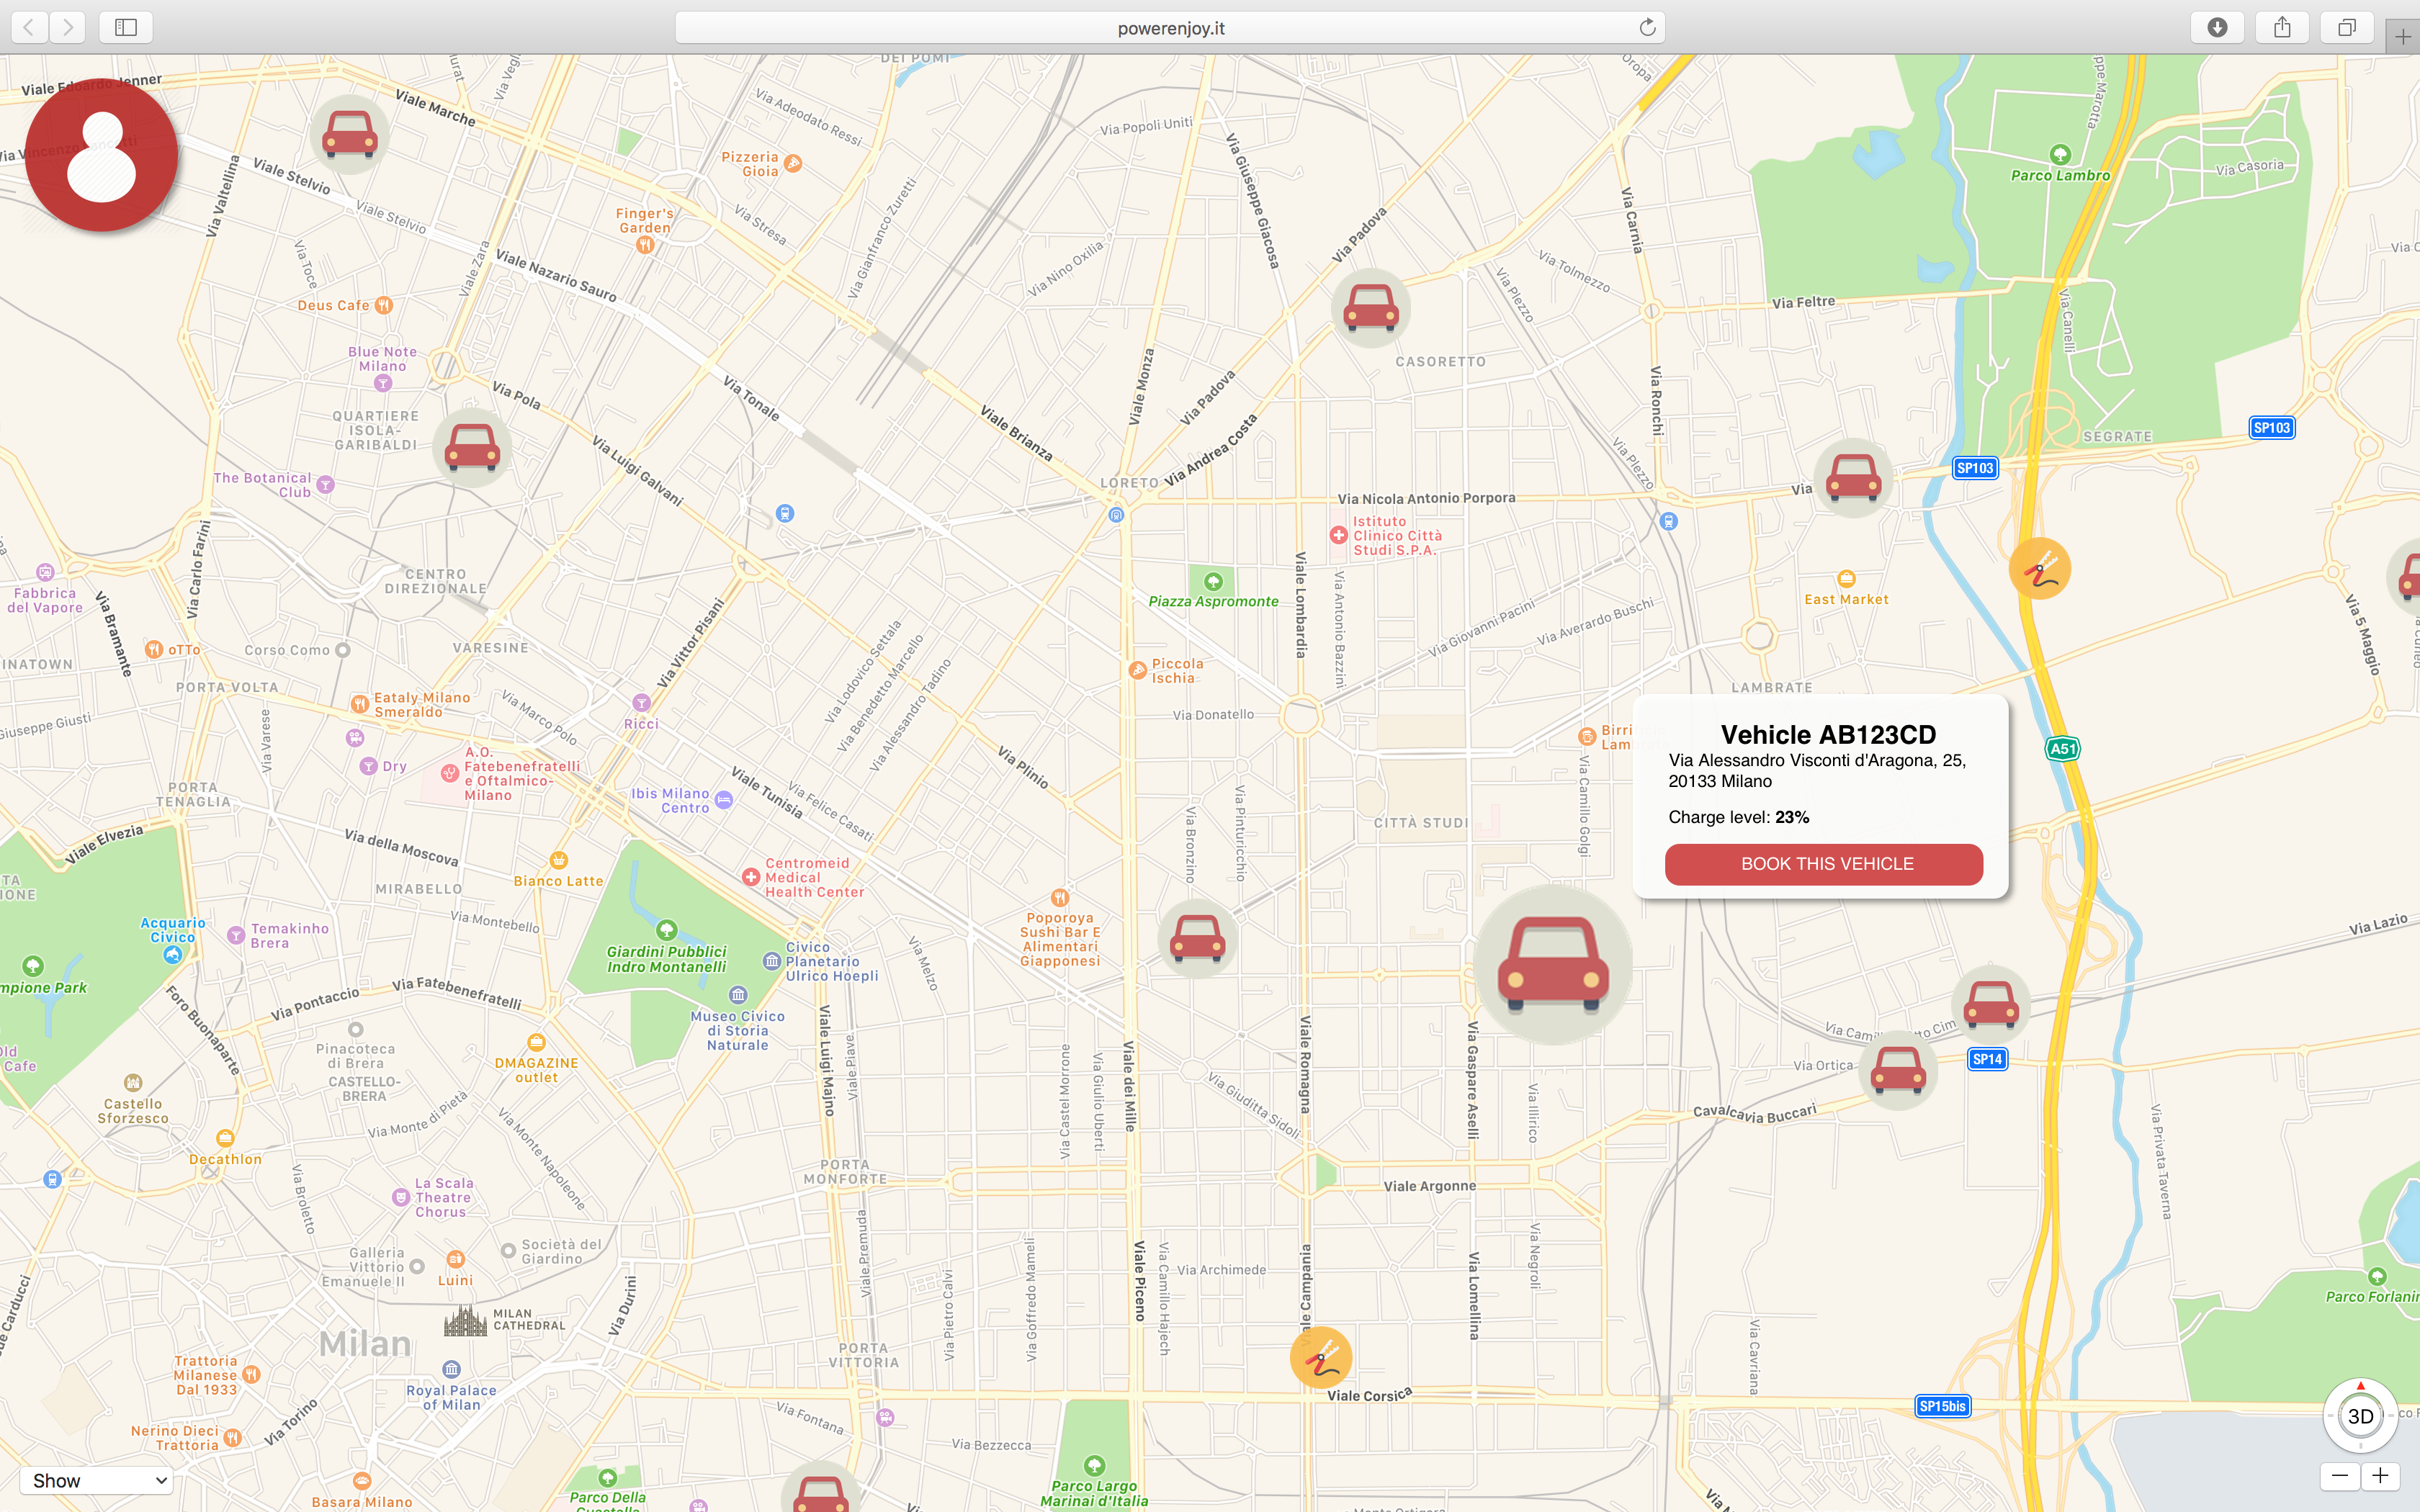
\includegraphics[width=1.0\textwidth]{/RASD/web_mockup}\\ 
	\vspace{0.5cm}
	\caption{1-page mockup representing the main page of the web application} \label{fig:web_mockup} 
\end{figure}

\newpage
\subsection{Hardware interfaces}
%gps and internet access from on-board computer
The on-board computer is equpped with a GPS. The  navigation system and the map data are supplied by the Navigation Data Standard (NDS). The road database is stored in an hard disk, other media may be added by the system via internet access. It can receive and display information on traffic congestion using either TMC and RDS.
The internet access is permitted by a USB modem with the Long-Term Evolution (LTE) standard that guarantee an high-speed wireless communication with the system.
The on-board computer is connected with a standard diagnostic connector and are using the car's OBD-II communication protocols for self-diagnostic and reporting capability.

\subsection{Software interfaces}
\begin{itemize}
	\item{Database Management System
		\begin{itemize}
			\item{{\bf Name}: MySQL}
			\item{{\bf Version}: 5.7.16}
			\item{{\bf Source}: http://www.mysql.com}
		\end{itemize}
	}
	\item{Java Virtual Machine
		\begin{itemize}
			\item{{\bf Name}: JEE}
			\item{{\bf Version}: 7}
			\item{{\bf Source}: http://www.oracle.com/technetwork/java/javaee}
		\end{itemize}
	}
	\item{Application Server
		\begin{itemize}
			\item{{\bf Name}: GlassFish}
			\item{{\bf Version}: 4.1.1}
			\item{{\bf Source}: https://glassfish.java.net}
		\end{itemize}
	}
	\item{Operating System
		\begin{itemize}
			\item{Application must be able to run on any SO which supports JVM and
				  DBMS specified before}
		\end{itemize}
	}

\end{itemize}

\subsection{API interfaces}
To provide location services we use the W3C Geolocation API combined with the GeoNames API for reverse geocoding. 
\\As well described on the producer's website, this combination gives us an accurate way to retrieve the user position for any location on Earth. 
\\The notifications email are handled using the Open-Source JavaMail API.
\\Regarding the payment method we use the Stripe API, that gives a secure and fast way to tranfer money. 
\\More information on dev.w3.org, geonames.org, www.oracle.com and stripe.com.

\subsection{Communication interfaces}
\begin{center}
	\begin{tabular}{|l|l|l|}
	    \hline
	    Protocol & Application & Port \\\hline
	    \hline
	    TCP & HTTP & 443 \\\hline
	    TCP & HTTPS & 80 \\\hline
	    TCP & DBMS & 3306(default) \\\hline
	\end{tabular}
\end{center}